\chapter{Implementacija i korisničko sučelje}
		
		
		\section{Korištene tehnologije i alati}
		
			Tim je koristio \underline{WhatsApp}.\footnote[1]{https://www.whatsapp.com/} i \underline{Notion}.\footnote[2]{https://www.notion.so/} za komunikaciju unutar tima. Za izradu UML dijagrama korišten je \underline{Astah Professional}.\footnote[3]{https://astah.net/products/astah-professional/}, dok je za upravljanje izvornim kodom odabran \underline{Git}.\footnote[4]{https://git-scm.com/}. Udaljeni repozitorij projekta dostupan je na web platformi \underline{GitHub}.\footnote[5]{https://github.com/}.
			
			Kao razvojna okruženja korišteni su \underline{Visual Studio Code}.\footnote[6]{https://code.visualstudio.com/} i \underline{IntelliJ IDEA}.\footnote[7]{https://www.jetbrains.com/idea/}. Visual Studio Code je jednostavan uređivač koda s podrškom za razvojne operacije poput debugiranja, pokretanja zadataka i kontrolu verzija od tvrtke Microsoft, dok je IntelliJ popularno razvojno okruženje (IDE) razvijeno od strane tvrtke JetBrains. Namijenjeno je prvenstveno za rad s Java programskim jezikom.
			
			Aplikacija je napisana koristeći radni okvir \underline{Spring Boot}.\footnote[8]{https://spring.io/projects/spring-boot/} i jezik \underline{Java}.\footnote[9]{https://www.java.com/en/} za izradu backenda te \underline{React}.\footnote[10]{https://react.dev/} i jezik \underline{JavaScript}.\footnote[11]{https://www.javascript.com/} za izradu frontenda. React je besplatna i open-source JavaScript biblioteka za izgradnju korisničkih sučelja temeljenih na komponentama. Održava je Meta i zajednica pojedinačnih razvijatelja te tvrtki. Radni okvir Spring Boot je otvoreni, mikroservisni Java web okvir koji nudi Spring. Razvijen je kako bi pojednostavio proces izrade, konfiguracije i razmještanja Java aplikacija. 
			
			Baza podataka se nalazi na posluzitelju u oblaku \underline{Render}.\footnote[12]{https://render.com/}.
			
			
			\eject 
		
	
		\section{Ispitivanje programskog rješenja}
			
			\textbf{\textit{dio 2. revizije}}\\
			
			 \textit{U ovom poglavlju je potrebno opisati provedbu ispitivanja implementiranih funkcionalnosti na razini komponenti i na razini cijelog sustava s prikazom odabranih ispitnih slučajeva. Studenti trebaju ispitati temeljnu funkcionalnost i rubne uvjete.}
	
			
			\subsection{Ispitivanje komponenti}
			\underline{\textbf{1. checkAnimalDto}}
			
			Jedna od komponenti koju smo testirali je metoda checkAnimalDto iz klase SearcherInTheFieldJpa. Ta metoda provjerava sadrži li animalDto sve potrebne varijable:
			\begin{lstlisting}
			public void checkAnimalDto(AnimalDto animalDto){
				if (animalDto == null) {
					throw new IllegalArgumentException("AnimalDto is null");
				}
				if (animalDto.getAnimalName() == null || animalDto.getAnimalName().isEmpty()) {
					throw new IllegalArgumentException("AnimalName is missing");
				}
				if (animalDto.getBreed() == null || animalDto.getBreed().isEmpty()) {
					throw new IllegalArgumentException("Breed is missing");
				}
				if (animalDto.getDescription() == null || animalDto.getDescription().isEmpty()) {
					throw new IllegalArgumentException("Description is missing");
				}
				if (animalDto.getCurrentPosition() == null || animalDto.getCurrentPosition().isEmpty()) {
					throw new IllegalArgumentException("Current position is missing");
				}
			}
			\end{lstlisting}
			Ako se neka od varijabli ne nalazi u animalDto, metoda baca exception ovisan o tome koja varijabla nedostaje. Metoda također provjerava je li sam animalDto prazan. Svi ispitni slučajevi ove metode nalaze se u klasi CheckAnimalDtoTest.\\
			
			\noindent\textbf{Prvi slučaj: testCheckAnimalDtoValid}
			
			Prvi slučaj koji se testira je kada je ulaz metode checkAnimalDto animalDto koji sadrži sve potrebne varijable:
			\begin{lstlisting}
				@Test
				public void testCheckAnimalDtoValid() {
					
					AnimalDto validAnimalDto = new AnimalDto();
					validAnimalDto.setAnimalName("Vuk");
					validAnimalDto.setBreed("Licki");
					validAnimalDto.setDescription("Sivi, brzi vuk");
					validAnimalDto.setCurrentPosition(Arrays.asList(1.0, 2.0));
					
					assertDoesNotThrow(() -> searcherJpa.checkAnimalDto(validAnimalDto));
				}
			\end{lstlisting}
			Taj slučaj na kraju ispituje je li bačen exception, tj. ako exception nije bačen onda test prolazi. Rezultat ispitnog slučaja je:
			
			\begin{figure}[H]
				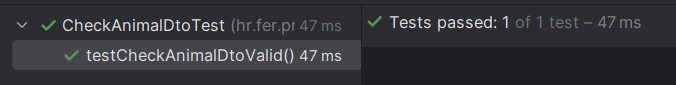
\includegraphics[scale=0.8]{slike/testCheckAnimalDtoValid.PNG} 
				\centering
				\caption{testCheckAnimalDtoValid rezultat}
				\label{fig:testCheckAnimalDtoValid}
			\end{figure}
			
			\noindent\textbf{Drugi slučaj: testCheckAnimalDtoNull}
			
			Također postoji slučaj koji testira da će se baciti ispravan exception ako je animalDto na ulazu prazan:
			\begin{lstlisting}
				@Test
				public void testCheckAnimalDtoNull() {
					AnimalDto nullAnimalDto = null;
					
					IllegalArgumentException exception = assertThrows(IllegalArgumentException.class,
					() -> searcherJpa.checkAnimalDto(nullAnimalDto));
					
					assertEquals("AnimalDto is null", exception.getMessage());
				}
			\end{lstlisting}
			Ako se baci exception da je animalDto prazan s porukom "AnimalDto is null", ispitni slučaj prolazi. Rezultat ispitnog slučaja je:
			
			\begin{figure}[H]
				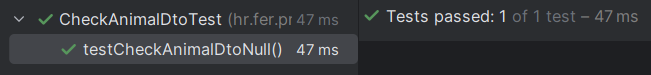
\includegraphics[scale=0.8]{slike/testCheckAnimalDtoNull.PNG} 
				\centering
				\caption{testCheckAnimalDtoNull rezultat}
				\label{fig:testCheckAnimalDtoNull}
			\end{figure}
			
			\noindent\textbf{Treći slučaj: testCheckAnimalDtoMissingName}
			
			Ovaj ispitni slučaj provjerava da će se baciti ispravan exception ako u objektu animalDto nedostaje varijabla imena:
			\begin{lstlisting}
				@Test
				public void testCheckAnimalDtoMissingName() {
					AnimalDto missingNameDto = new AnimalDto();
					missingNameDto.setBreed("Licki");
					missingNameDto.setDescription("Sivi, brzi vuk");
					missingNameDto.setCurrentPosition(Arrays.asList(1.0, 2.0));
					
					IllegalArgumentException exception = assertThrows(IllegalArgumentException.class,
					() -> searcherJpa.checkAnimalDto(missingNameDto));
					
					assertEquals("AnimalName is missing", exception.getMessage());
				}
			\end{lstlisting}
			Ovaj ispitni slučaj prolazi ako se baci exception s porukom "AnimalName is missing". Rezultat slučaja je:
			
			\begin{figure}[H]
				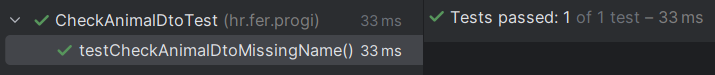
\includegraphics[scale=0.8]{slike/testCheckAnimalDtoMissingName.PNG} 
				\centering
				\caption{testCheckAnimalDtoMissingName rezultat}
				\label{fig:testCheckAnimalDtoMissingName}
			\end{figure}
			
			\noindent\textbf{Četvrti slučaj: testCheckAnimalDtoMissingBreed}
			
			Posljednji ispitni slučaj ove komponente sičan je trećem ispitnom slučaju, ali ovaj put provjerava da će metoda ispravno reagirati ako nedostaje varijabla Breed:
			\begin{lstlisting}
				@Test
				public void testCheckAnimalDtoMissingBreed() {
					AnimalDto missingBreedDto = new AnimalDto();
					missingBreedDto.setAnimalName("Vuk");
					missingBreedDto.setDescription("Sivi, brzi vuk");
					missingBreedDto.setCurrentPosition(Arrays.asList(1.0, 2.0));
					
					IllegalArgumentException exception = assertThrows(IllegalArgumentException.class,
					() -> searcherJpa.checkAnimalDto(missingBreedDto));
					
					assertEquals("Breed is missing", exception.getMessage());
				}
			\end{lstlisting}
			Slično kao u prijašnjem ispitnom slučaju, ako metoda baci exception s porukom "Breed is missing" ispitni slučaj prolazi. Rezultat ispitnog slučaja je:
			
			\begin{figure}[H]
				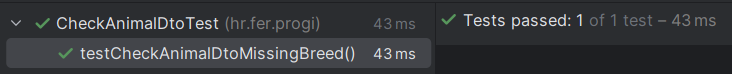
\includegraphics[scale=0.8]{slike/testCheckAnimalDtoMissingBreed.PNG} 
				\centering
				\caption{testCheckAnimalDtoMissingBreed rezultat}
				\label{fig:testCheckAnimalDtoMissingBreed}
			\end{figure}
			
			
			\underline{\textbf{2. putRemoveFromAction}}
			
			\underline{\textbf{3. checkRequestDto}}
			
			\underline{\textbf{4. validateCoordinates}}
			
			\underline{\textbf{5. checkAvailableSearcherDto}}
			
			
			\subsection{Ispitivanje sustava}
			
			 \textit{Potrebno je provesti i opisati ispitivanje sustava koristeći radni okvir Selenium\footnote{\url{https://www.seleniumhq.org/}}. Razraditi \textbf{minimalno 4 ispitna slučaja} u kojima će se ispitati redovni slučajevi, rubni uvjeti te poziv funkcionalnosti koja nije implementirana/izaziva pogrešku kako bi se vidjelo na koji način sustav reagira kada nešto nije u potpunosti ostvareno. Ispitni slučaj se treba sastojati od ulaza (npr. korisničko ime i lozinka), očekivanog izlaza ili rezultata, koraka ispitivanja i dobivenog izlaza ili rezultata.\\ }
			 
			 \textit{Izradu ispitnih slučajeva pomoću radnog okvira Selenium moguće je provesti pomoću jednog od sljedeća dva alata:}
			 \begin{itemize}
			 	\item \textit{dodatak za preglednik \textbf{Selenium IDE} - snimanje korisnikovih akcija radi automatskog ponavljanja ispita	}
			 	\item \textit{\textbf{Selenium WebDriver} - podrška za pisanje ispita u jezicima Java, C\#, PHP koristeći posebno programsko sučelje.}
			 \end{itemize}
		 	\textit{Detalji o korištenju alata Selenium bit će prikazani na posebnom predavanju tijekom semestra.}
			
			\eject 
		
		
		\section{Dijagram razmještaja}
			
			\textbf{\textit{dio 2. revizije}}
			
			 \textit{Potrebno je umetnuti \textbf{specifikacijski} dijagram razmještaja i opisati ga. Moguće je umjesto specifikacijskog dijagrama razmještaja umetnuti dijagram razmještaja instanci, pod uvjetom da taj dijagram bolje opisuje neki važniji dio sustava.}
			
			\eject 
		
		\section{Upute za puštanje u pogon}
		
			\textbf{\textit{dio 2. revizije}}\\
		
			 \textit{U ovom poglavlju potrebno je dati upute za puštanje u pogon (engl. deployment) ostvarene aplikacije. Na primjer, za web aplikacije, opisati postupak kojim se od izvornog kôda dolazi do potpuno postavljene baze podataka i poslužitelja koji odgovara na upite korisnika. Za mobilnu aplikaciju, postupak kojim se aplikacija izgradi, te postavi na neku od trgovina. Za stolnu (engl. desktop) aplikaciju, postupak kojim se aplikacija instalira na računalo. Ukoliko mobilne i stolne aplikacije komuniciraju s poslužiteljem i/ili bazom podataka, opisati i postupak njihovog postavljanja. Pri izradi uputa preporučuje se \textbf{naglasiti korake instalacije uporabom natuknica} te koristiti što je više moguće \textbf{slike ekrana} (engl. screenshots) kako bi upute bile jasne i jednostavne za slijediti.}
			
			
			 \textit{Dovršenu aplikaciju potrebno je pokrenuti na javno dostupnom poslužitelju. Studentima se preporuča korištenje neke od sljedećih besplatnih usluga: \href{https://aws.amazon.com/}{Amazon AWS}, \href{https://azure.microsoft.com/en-us/}{Microsoft Azure} ili \href{https://www.heroku.com/}{Heroku}. Mobilne aplikacije trebaju biti objavljene na F-Droid, Google Play ili Amazon App trgovini.}
			
			
			\eject 